\documentclass[answers, a4paper, 11pt]{exam}
\usepackage{amsmath}
\usepackage{amssymb}
\usepackage{amsthm}
\usepackage[italian]{babel}
\usepackage{ccicons}
\usepackage{hyperref} % Has to be loaded before cleveref
\usepackage{cleveref}
\usepackage[utf8]{inputenc} % Has to be loaded before csquotes
\usepackage[autostyle=false, style=english]{csquotes}
\usepackage[margin=2cm]{geometry}
\usepackage{graphicx}
\usepackage{mathrsfs}
\usepackage{multicol}
\usepackage{relsize}
\usepackage{parskip}

\pagestyle{plain} 
\graphicspath{{./images/}}
\MakeOuterQuote{"}
\setlength{\columnseprule}{.4pt}
\renewcommand{\solutiontitle}{\noindent\textbf{R:}\enspace}
\def\dbar{{\mathchar'26\mkern-12mu d}}

\title{Ingegneria del Software T}
\author{Kevin Michael Frick}
\begin{document}
\maketitle
\textbf{Disclaimer}:  Questo disclaimer, di solito, lo metto alla fine. 
Ma questa volta siamo nel 2020 e la COVID-19 è una realtà, così come gli esami online, quindi ho pensato che fosse il caso di assicurarmi che tu lo leggessi (legga? boh, dopo tre anni di ingegneria mi sto scordando l'italiano).
Lo so che hai notato che il docente del corso, durante la simulazione, non ha mostrato di preoccuparsi particolarmente di cosa ci fosse nella stanza intorno a te.
Quindi, forse, sei tentat@ di stamparti questo file, nasconderlo chissà dove e, come disse un vecchio saggio, \textit{copiare come un animale} durante l'esame. 
È comodo e facile, no? 
\textit{E poi, Kevin, non fai questi file proprio perché vuoi che i professori si accorgano che non è il caso di fare sempre le stesse domande?}

Già. 
Li faccio per questo motivo. 
Però se tutt@ scrivono esattamente quello che c'è scritto in questo file, il docente lo noterà subito, capirà cosa è successo e potrebbe invalidare la prova. 
E ovviamente alla prossima prova farà attenzione che nessun@ copi, obbligandoci a mettere cinque webcam in giro per la stanza e una in cucina perché non si sa mai. 
Se invece userai questo file come aiuto per lo studio, è comunque probabile che andrai bene all'esame (perché \href{https://www.ernweb.com/educational-research-articles/learning-techniques-effective-study/}{allenarsi a rispondere alle domande è un metodo molto efficace per studiare}) e questo materiale lo imparerai davvero.

Ed è importante che impari davvero il materiale di questo corso, così come quello di qualunque altro corso universitario. 

Questo è un corso del terzo anno. 
È ragionevole pensare che a breve ti laureerai e andrai a lavorare come ingegnere informatico, e non siamo più nel 1965: i sistemi informatici sono critici quanto ponti e strade.
Se i sistemi informatici falliscono, la gente muore.
\href{https://en.wikipedia.org/wiki/Boeing_737_MAX_groundings}{Pensa al caso dei Boeing 737 MAX.}

Quindi, per favore, non copiare.
Oppure, un giorno, un sistema informatico mal progettato potrebbe uccidere te o persone a te care.
E in ogni caso, ricorda:

\textit{Questo documento può contenere errori e imprecisioni che potrebbero danneggiare sistemi informatici, terminare relazioni romantiche e rapporti di lavoro, portare i gatti a liberare le proprie vesciche sulla moquette e causare un conflitto termonucleare globale.
Procedere con cautela.}

\begin{questions}

\question \textbf{Processo di sviluppo del software}
\begin{parts}
\part
Processo di sviluppo a cascata.
\begin{solution}
Le fasi di sviluppo di un software sono definizione, progettazione, sviluppo e manutenzione.

La fase di definizione concerne la discussione con il committente e l'analisi/ingegneria dei requisiti. Questa fase è seguita dalla progettazione, durante la quale viene progettato un sistema software che risponde ai requisiti del committente. Durante la fase di sviluppo la soluzione progettata viene effettivamente implementata. La fase di manutenzione comprende il deployment, l'addestramento degli utilizzatori e la correzione di eventuali errori nel codice.

Nel processo di sviluppo a cascata queste fasi si susseguono senza retroazione: dopo approfondite discussioni con il committente viene redatto un documento di progetto quanto più completo e dettagliato possibile, il quale viene seguito pedissequamente dagli implementatori. Una volta eseguito il deployment e addestrati gli utenti, si mette mano al codice solo per correggere eventuali errori.

Lo sviluppo a cascata presenta notevoli criticità: l'assenza di retroazione tra le fasi significa che non è possibile  modificare un prodotto delle fasi precedenti, ma nella realtà i requisiti come formulati dal committente sono spesso vaghi e/o richiedono chiarimenti nelle fasi di progettazione. Allo stesso modo, il deployment di un particolare componente potrebbe essere reso molto più semplice da una modifica nella struttura del suo codice, o gli utenti potrebbero far notare che l'interfaccia utente è difficile da utilizzare.

L'assenza di retroazione nel modello a cascata deriva dalla volontà di ridurre i costi impiegando il personale richiesto da ogni fase per il minor tempo possibile: per questo motivo, nonostante esistano versioni del modello a cascata con limitata retroazione, spesso il costo dell'introduzione di quest'ultima più che compensa i risparmi permessi dal modello a cascata. 
\end{solution}
\part Revisione black box e white box.
\begin{solution}
Il collaudo delle funzionalità di un sistema, così come quello della sua sicurezza, può avvenire seguendo un approccio a black box e a white box.

La revisione black box è mirata a collaudare le proprietà del sistema che sono visibili dall'esterno e che possono essere apprezzare senza conoscere il funzionamento del software: affidabilità, semplicità d'uso, velocità ecc.
Nel caso dei test di sicurezza, il collaudatore si mette nei panni dell'attaccante e cerca di penetrare nel sistema sfruttando le conoscenze che si possono avere semplicemente guardando il sistema. 

La revisione white box invece è mirata ad analizzare la struttura interna del software e valutare caratteristiche come modularità e leggibilità del codice.
Queste caratteristiche sono un modo per realizzare le proprietà esterne e ne influenzano la qualità.
Nel caso dei test di sicurezza, il test white box consiste nell'analisi del codice e nella scrittura di test molto specifici che sfruttano le caratteristiche del codice per violare il sistema. 
\end{solution}
\part Rational Unified Process
\begin{solution}
Le fasi di processo di sviluppo di un software sono specifica, sviluppo, validazione ed evoluzione.
RUP è un modello di processo di sviluppo iterativo unificato, che contiene al suo interno tutti i modelli di processo: qualsiasi modello di processo può essere visto come parte di RUP.
È un modello ibrido quindi può comportarsi come qualunque altro modello.
Definisce delle direttive che possano essere realizzate e implementate in modo da realizzare diversi processi. Una certa azienda può usare RUP per un processo vicino a quello evolutivo, oppure a componenti ecc.
È pensato per progetti di grandi dimensioni perché ha una parte formale abbastanza importante.
RUP vede il processo da tre prospettive ortogonali: 
\begin{enumerate}
\item Prospettiva dinamica: far vedere come il modello si sviluppa nel tempo.
Divisa in:
\begin{itemize}
\item  Avvio = analisi di fattibilità. Il suo scopo è definire in maniera accurata, non ambigua quale sia l'ambito in cui ci si muove. Esempi: il tipo di mercato, gli attori e i sistemi che interagiranno. Si usano modelli di casi d'uso e una serie di modelli formali.
\item Elaborazione: racconta come il sistema sarà fatto, includendo l'analisi del dominio e buona parte della progettazione, dove non necessariamente si arriva a specificare i componenti ma quantomeno a specificare l'architettura generale del sistema.
Modello dei casi d'uso, descrizione architettura, sviluppo di un prodotto eseguibile. Questa fase di elaborazione rivede quanto è previsto nella fase di avvio. 
\item  Costruzione: parte finale della progettazione, seguita da sviluppo e test. 
\item  Transizione: deployment, manutenzione, addestramento degli utenti, eventuale retroazione. 
\end{itemize}
Tutte queste quattro fasi possono avere retroazioni alle fasi precedenti, non necessariamente immediatamente precedenti. 
\item Prospettiva statica: quali sono le attività da realizzare all'interno del progetto. 
Queste attività si chiamano "workflow", da non confondere con la visione dinamica: non è detto che i requisiti, ad esempio, si analizzino nella fase di inizio.
Questo è vero solo nel modello a cascata, ma non ad esempio in quello iterativo. 
Si ha separazione tra tempo e attività svolte. 
Esisono sei workflow principali e tre di supporto: ci dovrebbero essere nove entità nell'azienda, all'interno delle quali ognuno ha un compito specifico. 
Ogni workflow ha un modello UML associato.
Tutti i workflow possono essere attivi in ogni stadio del processo. 
I workflow sono;
\begin{enumerate}
    \item Modellazione delle attività aziendali: i processi che sono all'interno dell'azienda vengono modellati come UML use case;
    \item Requisiti: identificano quali siano gli attori che partecipano al sistema e racconta come sia fatta l'interazione col sistema, servendosi degli UML use case;
    \item Analisi e progetto: si crea il modello di progetto. 
    UML, per questa fase, definisce vari modelli: architetturali, componenti, a oggetti, sequenziali.
    \item Implementazione: saranno interessati gli implementatori, e se l'analisi del progetto è stata fatta usando i modelli UML è possibile generare automaticamente codice oppure in ogni caso UML rende facile il trasferimento di specifiche dalla fase di progetto all'implementazione.
    \item Test: dei sottosistemi e del sistema finale;
    \item Rilascio. 
\end{enumerate}
I tre workflow di supporto, che sono ortogonali alla fase di sviluppo e ai sei principali e adottabile da ciascuno di essi, sono:
\begin{enumerate}
    \item Gestione delle modifiche: gestisce il cambiamento (es. diverse versioni del software), non solo del software ma anche dei modelli;
    \item Gestione del progetto: personale, costi, ecc. Supporto in toto allo sviluppo;
    \item Ambiente: si occupa degli strumenti utilizzati per progettare e implementare (disegni UML, IDE, ecc).
\end{enumerate}
\item Prospettiva pratica: definisce le "buone prassi" da seguire durante il processo. Sono idee che sono già note all'interno dell'azienda.
Divisa in sei pratiche fondamentali, sei regole che dovrebbero sempre guidare il processo di sviluppo. 
I design pattern / principle derivano da queste pratiche. 
\begin{enumerate}
    \item Sviluppo ciclico: il modello a cascata va bene, ma deve esserci retroazione.
    Fin da subito vanno mostrate al cliente le parti del software che soddisfano i requisiti più importanti. 
    \item Gestione dei requisiti = documentazione: usare modelli per la specifica dei requisiti, condividerli con i clienti e farli accettare da loro.
    \item Usare architetture basate su componenti: riutilizzare parti di software già scritti rende l'architettura del sistema più modulare  ùindi più facilmente modificabile emanutenibili.
    \item Creare modelli visivi del software: scrivere il codice non basta e ci vuole una visualizzazione di tutte le fasi di produzione del software.
    Non è un caso che UML sia stato sviluppato insieme a RUP, perché deriva proprio da questa prospettiva pratica. 
    I modelli UML permettono di capire velocemente che cosa farà il software. 
    Questi modelli devono mostrare sia il comportamento statico che quello dinamico del software. 
    \item Verificare la qualità: ci devono essere delle misure che dicano se il software soddisfa o meno degli standard di qualità, che devono essere definiti all'interno dell'azienda.
    \item Controllare le modifiche: utilizzare degli strumenti e delle pratiche che permettano di gestire modifiche, configurazioni ecc. 
\end{enumerate}
\end{enumerate}
Le varie fasi procedono per iterazioni: le iterazioni iniziali della fase di avvio ad esempio usano molto il workflow dei requisiti, così come quella di elaborazione, mentre è meno usato dalla fase di costruzione. 
\end{solution}
\end{parts}

\question \textbf{Analisi e progettazione orientata agli oggetti: linguaggi di modellazione, UML.}
\begin{parts}
\part Polimorfismo secondo Cardelli-Wegner
\begin{solution}
Il polimorfismo è la capacità di uno stesso elemento di assumere forme diverse in contesti diversi, o di elementi diversi di assumere la stessa forma in un determinato contesto.
La classificazione Cardelli-Wegner dei polimorfismi li divide in due macro-categorie, universali e ad-hoc.

Gli elementi universalmente polimorfici possono assumere un numero infinito di forme. 
Questo si osserva, nella programmazione orientata agli oggetti, nel \textit{polimorfismo per inclusione}, rappresentato dall'overriding dei metodi e dal binding dinamico delle funzioni.
Il polimorfismo universale si osserva inoltre nella programmazione generica rispetto ai tipi, che esprime il \textit{polimorfismo parametrico}: si definisce una classe in cui il tipo di una o più variabili è un parametro della classe stessa.
Da ogni classe generica vengono generate classi indipendenti, che non hanno un rapporto di ereditarietà. 

Un elemento polimorfico ad-hoc, invece, può assumere un numero finito di forme.
Ciò si osserva nell'\textit{overloading} di funzioni e operatori, che richiede una ridefinizone per ogni insieme di argomenti accettati.
Il polimorfismo ad-hoc si osserva inoltre nella \textit{coercion}, quando una variabile di un certo tipo viene convertita, esplicitamente o implicitamente, a un tipo diverso.
Anche in questo caso, le conversioni possibili devono essere definite una per una in fase di programmazione.
\end{solution}

\end{parts}

\question \textbf{Analisi dei requisiti: raccolta dei requisiti e loro validazione, analisi del dominio, analisi dei requisiti, casi d'uso e scenari.}
\begin{parts}
\part Tipologie di requisiti
\begin{solution}Vi sono tre tipologie di requisiti:
\begin{enumerate}
    \item Requisiti funzionali: descrivono cosa fa il sistema, ma non come lo fa. 
    Sono un elenco di servizi che il sistema deve fornire. 
    In particolare, per ciascuno di questi servizi, bisogna indicare come gli input fanno reagire il sistema e come si comporta in alcune situazioni.
    Descrivono anche cosa \textit{non} deve fare il sistema in precise situazioni. 
    Le specifiche devono essere complete, ovvero definire tutti i servizi forniti, e coerenti, cioè non essere in contraddizione tra loro. 
    \item Requisiti non funzionali: descrivono altre caratteristiche del sistema, ad esempio quali siano le proprietà del sistema (requisiti del prodotto), vincoli di sviluppo (requisiti organizzativi) o vincoli derivanti da altri sistemi esterni o contesti legislativi/etici (requisiti esterni).
    I requisiti non funzionali tendenzialmente sono espressi in modo vago. 
    Inoltre, vengono spesso mescolati con i requisiti non funzionali o si contraddicono tra di loro. 
    \item Requisiti di dominio: derivano dal dominio di applicazione del sistema e indicano come il sistema debba funzionare all'interno di un certo dominio, e raccontano certi requisiti che sono specifici del dominio.
    Dovrebbero raccontare a progettisti quale sia il dominio di applicazione del sistema, che spesso non è chiaro al progettista.
\end{enumerate}\end{solution}
\end{parts}

\question \textbf{Progettazione: progettazione dell’architettura del sistema.}
\begin{parts}

\part Principi per l'architettura dei package.
\begin{solution}
Vi sono tre principi che guidano la progettazione dell'architettura dei package:
\begin{itemize}
    \item Il principio di equivalenza riuso/rilascio (reuse/release equivalence principle) afferma che la granularità del riuso e del rilascio debbano coincidere.
    Se si ha un elemento che deve essere riutilizzato, esso deve essere periodicamente rilasciato/fornito: chi realizza il software non è chi lo usa. 
    Se non si è in grado di garantire che il software venga mantenuto, nessuno lo utilizzerà.
    Il motivo per il quale le classi si raggruppano in package è il riutilizzo: se si vogliono riutilizzare certi elementi, essi vanno raggruppati in package.
    \item Il principio di chiusura comune (common closure principle) afferma che le classi che vengono modificate assieme debbano essere incluse nello stesso package. 
    Siccome, all'interno di un progetto SW, ogni volta che viene modificato un package l'intero package va ridistribuito, e tutti gli utilizzatori devono aggiornarlo, è importante minimizzare il numero di package che cambiano quando si cambia una classe. 
    \item Il principio di riutilizzo comune (common reuse principle) afferma che le classi che non vengono riutilizzate insieme non vadano incluse nello stesso package.
    Ciò complementa il CCP, ma non ne è implicato: deriva invece dal fatto che una dipendenza da una classe in un package porta con se una dipendenza dall'intero package. 
\end{itemize}

È difficile soddisfare tutti e tre i principi contemporaneamente: il primo e il terzo tendono a facilitare l'utilizzo dei package da parte dei clienti mentre il secondo tende a semplificare l'utilizzo dei package da parte dello sviluppatore. 
Il CCP tende a suggerire di creare package molto grandi, mentre il RREP e il CRP tendono a suggerire package molto piccoli.
Per questo motivo, normalmente si cerca di soddisfare il CCP, e una volta che l'architettura dei package si stabilizza si esegue un refactor per rimpicciolire i package e soddisfare gli altri due principi.
In questo modo, all'inizio si facilita il lavoro agli sviluppatori, e in seguito per aumentare la vita utile del SW si applicano gli altri due principi. 

Vi sono inoltre tre principi che descrivono le relazioni tra i package:
\begin{itemize}
    \item Il principio delle dipendenze acicliche afferma che vadano evitati cicli di dipendenze tra package: dato che modificare una classe richiede di ricompilare il package a cui appartiene quella classe e tutti i package che dipendono da esso, una singola dipendenza ciclica può portare alla necessità di ricompilare l'intero progetto se si cambia una sola classe. 
    È possibile rompere un ciclo spostando la dipendenza da una classe esterna al package a una interfaccia definita all'interno del package e implementata dalla classe, ma non è sempre questa la soluzione;
    \item Il principio delle dipendenze stabili afferma che un package dovrebbe dipendere solo da package più stabili di esso. 
    Un package dal quale dipendono molti altri package non può essere volatile, e al contrario i package che cambiano spesso non possono avere molte dipendenze, per evitare che diventi necessario ricompilare molto spesso tutte queste dipendenze. 
    Per ottenere dipendenze stabili ci si conforma al CCP: se molte classi dipendono da una classe, questa e le sue dipendenze vanno tutte inserite nello stesso package e ricompilate assieme, evitando in questo modo effetti a cascata;
    \item Il principio delle astrazioni stabili afferma che i package stabili dovrebbero essere package astratti.
    Ciò significa che un modo per ottenere stabilità è rendere astratti gli elementi che si vuole siano stabili: un package astratto non ha codice al suo interno che possa cambiare. 
\end{itemize}

Il principio di stratificazione unisce questi ultimi tre principi: un sistema di package a livelli non ha cicli e permette di posizionare i package più instabili in alto, in modo che abbiano poche dipendenze entranti, e i package più stabili - tendenzialmente astratti - in basso, in modo che possano avere molte dipendenze entranti. 
\end{solution}
\end{parts} 

\question \textbf{Principi di progettazione}
\begin{parts}
\part Rigidità, fragilità, viscosità e immobilità del software.
\begin{solution}
La qualità di un dato progetto potrebbe dipendere da vari fattori, principalmente dalle priorità organizzative. 
Utilizzare principi che rendono il codice manutenibile, a valle spesso si migliora anche affidabilità, efficienza e sicurezza.
Definire cosa rende un software mantenibile, però, è molto più complesso che definire cosa rende un software difficile da mantenere.
\begin{itemize}
\item Un software è rigido quando un singolo cambiamento apportato a una singola parte del progetto ha effetto su tante altre parti del sistema, e modificare un componente porta a dover modificare molti altri componenti.
L'effetto della rigidità si vede quando i dirigenti, se sanno che il SW è rigido, tenderanno di impedire agli sviluppatori di effettuare modifiche, anche piccole, perché non sanno quando gli sviluppatori finiranno effettivamente di modificare il SW.
\item Un software è fragile quando una modifica di una parte del progetto ha effetto su parti del sistema che non era previsto interessasse e che sembrano non essere correlate.
L'effetto della fragilità si vede quando i dirigenti non permettono agli sviluppatori di modificare il SW perché temono che tali modifiche inficino il funzionamento di tutto il sistema. 
\item Un software è immobile quando il codice non è utilizzabile in altre applicazioni, ad esempio perché porta con sé troppe dipendenze oppure perché richiede troppo tempo per essere adattato al nuovo, specifico caso d'uso. 
Come effetto di software immobile, gli sviluppatori perdono molto tempo a riscrivere, inutilmente,  pezzi di SW che sono già stati scritti. 
\item Un software è viscoso quando fare modifiche al software, anche piccole, porta a fare qualcosa di "sbagliato". 
In un software viscoso è facile fare la cosa sbagliata e difficile fare la cosa giusta.
Uno sviluppatore, normalmente, effettua modifiche a un software nel modo meno costoso: è possibile che il modo in cui è scritto il SW assicuri che il metodo meno costoso sia anche quello che meglio preserva il progetto iniziale, oppure no.
Se il progetto è viscoso in partenza, allora è più complicato preservarlo che mettere una "toppa".
Ciò può capitare anche se tutto l'ambiente di sviluppo è macchinoso, lento e inefficiente. 
L'effetto della viscosità è un visibile degrado della manutenibilità, che porta con il tempo a software rigido, fragile e immobile. 
\end{itemize}

Il software può essere mal progettato per le ridotte capacità dei progettisti, per l'obsolescenza delle tecnologie utilizzate, per limiti imposti che riguardano il tempo da spendere o le risorse da utilizzare, o a causa di un dominio troppo complesso. 

Inoltre, il SW può diventare mal progettato per motivi meno ovvi: la "marcescenza" del software è un processo lento. 
I requisiti possono cambiare in maniera inaspettata, e se i cambiamenti sono molto forti il software può smettere di essere valido.
Un esempio di una situazione simile è la necessità di mantenere la retrocompatibilità tra versioni successive di un SW. 
Infine, talvolta gli implementatori potrebbero aggiungere dipendenze non pianificate, che vanno gestite accuratamente. 
\end{solution}
\part Principio di sostituibilità di Liskov.
\begin{solution}
Il principio di sostituibilità di Liskov è un principio di programmazione orientata agli oggetti che definisce il rapporto tra una classe e le sue sottoclassi.
È possibile enunciare una "versione debole" del principio: a ogni variabile che fa riferimento alla classe base deve poter essere assegnato un riferimento di una sottoclasse.
Questa versione, però, non coincide con l'effettiva formulazione del principio, che è molto più forte.
Il principio afferma che ogni programma che utilizzi istanze della classe base deve poter utilizzare istanze delle sottoclassi senza che il comportamento logico del programma cambi.
Ciò significa che, per ogni metodo re-implementato dalla sottoclasse:
\begin{itemize}
    \item le precondizioni devono essere uguali o meno stringenti;
    \item le postcondizioni devono essere uguali o più stringenti;
    \item la semantica della classe base deve essere mantenuta;
    \item non è possibile aggiungere vincoli comportamentali alla classe base.
\end{itemize}

Ad esempio, un Quadrato è un Rettangolo ma aggiunge un vincolo: quando viene modificata l'altezza viene modificata anche la larghezza. 
Ciò significa che una modifica a una dimensione comprende un cambiamento nello stato dell'oggetto che non avviene invece nella superclasse, quindi un Quadrato non può essere sostituibile secondo Liskov a un Rettangolo.

Un altro modo per esprimere il principio è affermare che ogni sottoclasse onori lo stesso "contratto" della classe base, con riguardo alle postcondizioni e alle precondizioni. 
\end{solution}
\part Open/Close Principle
\begin{solution}
L'Open/Close Principle è un principio di programmazione che agevola la scrittura di software riutilizzabile.
L'OCP afferma che le entità software (classi, package ecc) dovrebbero essere aperte alle estensioni ma chiuse alle modifiche. 
Ciò significa che le entità possono essere estese aggiungendo nuovo stato o nuovo comportamento, ma l'interfaccia non deve essere modificabile: è ben definita, pubblica e statica.
Una volta chiusa e definita l'interfaccia, l'interno dell'entità può essere modificata a piacimento.
Ciò permette di modificare/estendere l'oggetto senza che il funzionamento sia affetto dalle modifiche. 
Per realizzare l'OCP si ricorre all'incapsulamento e all'astrazione: si definisce per prima cosa un'interfaccia stabile, che può poi essere estesa definendo, ad esempio, una classe concreta che implementa quell'interfaccia.
\end{solution}
\part Dependency inversion principle
\begin{solution}
Il principio di inversione delle dipendenze afferma che le dipendenze debbano essere relative ad astrazioni e non a implementazioni concrete. 
La direzione della specializzazione, quindi, dovrebbe essere verso una classe astratta o un'interfaccia e non verso una classe concreta. 
I moduli di alto livello non dovrebbero dipendere da quelli di basso livello, bensì entrambi dovrebbero dipendere da astrazioni: il cliente deve interrogare le astrazioni e il fornitore di servizio implementarle. 

Tendenzialmente, i moduli di basso livello sono i più soggetti ai cambiamenti, in quanto contengono codice più complesso. 
Se i requisiti cambiano o è necessario correggere un errore e si modificano i moduli di basso livello, tutti i moduli che ne dipendono devono essere modificati, causando rigidità, dato che bisogna intervenire su un alto numero di moduli, fragilità, perché si ha la potenzialità di introdurre errori in più parti del sistema,  e immobilità, perché non si può riutilizzare il codice perché porta con sé troppe dipendenze. 

Se i moduli di basso livello realizzano le interfacce e quelli di alto livello dipendono dalle interfacce, che sono stabili, è possibile modificare i moduli di basso livello senza modificare nulla nel codice dei moduli di alto livello. 
Le interfacce dei componenti vanno definite in anticipo, in analisi, in modo da garantire stabilità delle interfacce. 

Il principio funziona perché le astrazioni contengono poco codice e quindi sono poco soggette a cambiamenti. 
I cambiamenti non si propagano oltre il "muro" di astrazioni (design for change) e i moduli, disaccoppiati, facilitano il riutilizzo.
\end{solution}
\part Single responsibility principle
\begin{solution}
Il principio di singola responsabilità afferma che una classe debba avere una sola responsabilità e che ci debba sempre essere al massimo un solo motivo per modificare una classe.
Non appena una classe ha più di una responsabilità, esse diventano accoppiate e una modifica ad una richiede di modificare l'altra, portando a progetti fragili e poco riutilizzabili.
Nel caso una classe si trovi ad avere più responsabilità, va effettuato un refactoring per separare la classe in due, assegnando a ciascuna una responsabilità. 
\end{solution}
\part Interface segregation principle
\begin{solution}
Il principio di segregazione delle interfacce "estende" il principio di singola responsabilità affermando che i clienti non debbano dipendere da interfacce che non usano.
Ciò significa che, al momento della scrittura di un'interfaccia, è necessario minimizzarne i contenuti: avere tante interfacce specifiche è meglio che averne una sola (\textit{fat interface}) che fa molte cose. 

\end{solution}
\end{parts}
\question \textbf{Design pattern.}
\begin{parts}
\part Pattern singleton
\begin{solution}

\textbf{Problema:} Va garantita l'esistenza di al più una istanza di una classe, alla quale deve essere possibile accedere. 
Se esiste già una istanza di quella classe, allora è necessario intercettare tutte le richieste di creazione di una nuova istanza.

\textbf{Soluzione:} Si rende privato o protected il costruttore della classe.
All'interno della classe si inserisce un membro statico con lo stesso tipo della classe.
Si definisce un metodo statico \texttt{GetInstance()} che crea una istanza se non è già stata creata e la restituisce.

\textbf{Conseguenze:} non si può chiamare \texttt{new Singleton()} e si accede all'istanza solo tramite \texttt{GetInstance()}.

Una classe statica con solo membri statici non è una buona alternativa al pattern singleton, perché quest'ultimo permette di specializzare il metodo \texttt{GetInstance()} e restituire istanze specializzate, a seconda del contesto.
Inoltre, una classe singleton non statica può implementare un numero arbitrario di interfacce.

\textbf{Diagramma UML}:

{\centering

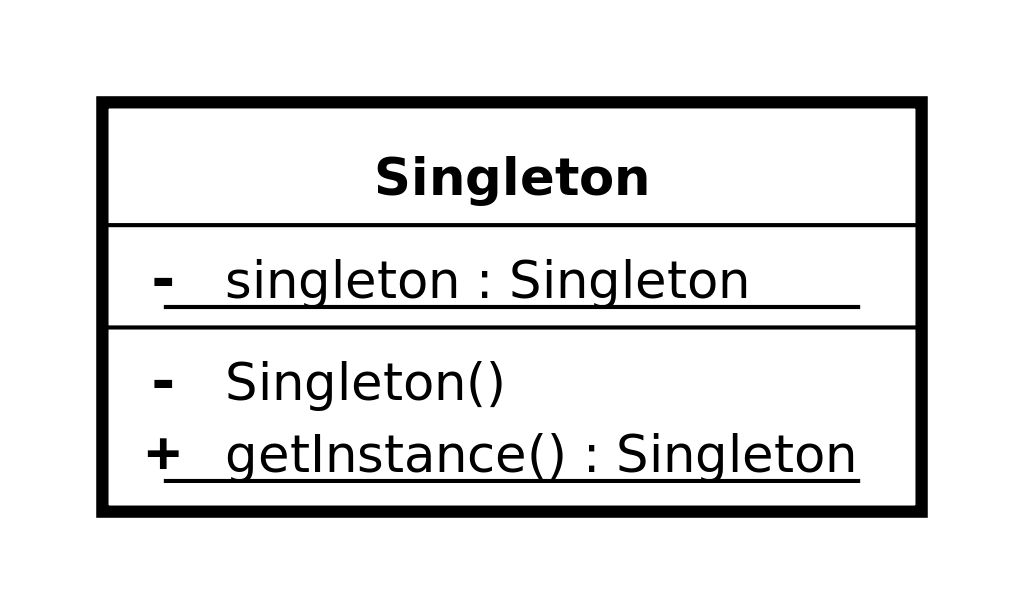
\includegraphics[width=0.4\textwidth]{Singleton}

}

\end{solution}

\part Pattern observer
\begin{solution}

\textbf{Problema:} Si ha un \texttt{Subject} le modifiche al quale devono ripercuotersi su uno o più \texttt{Observer}. 
Non si vuole scrivere nel codice del Subject l'aggiornamento degli Observer perché ciò richiederebbe la conoscenza reciproca, portando a un accoppiamento forte tra le parti e a codice difficile da riutilizzare.

\textbf{Soluzione:} Si imposta una relazione uno-a-molti tra \texttt{Subject} e \texttt{Observer}. 
Si definisce una clsse astratta \texttt{Subject} che dichiara i metodi \texttt{Attach()} (o \texttt{Register()}), \texttt{Detach()} (o \texttt{Unregister()}) e \texttt{Notify()}.
Si definisce inoltre una classe astratta \texttt{Observer} che dichiara il metodo \texttt{Update()}.
Un \texttt{Observer} si registra presso il \texttt{Subject} chiamando \texttt{Attach()}.
\texttt{Notify()} chiama \texttt{Update()} di tutti gli \texttt{Observer} che si sono registrati. 

\textbf{Conseguenze}: Obbliga a implementare in tutti gli \texttt{Observer} metodi per gestitre ogni tipo di modifica, anche se a un dato \texttt{Observer} ne interessano solo alcune. 

\textbf{Diagramma UML}:

{\centering

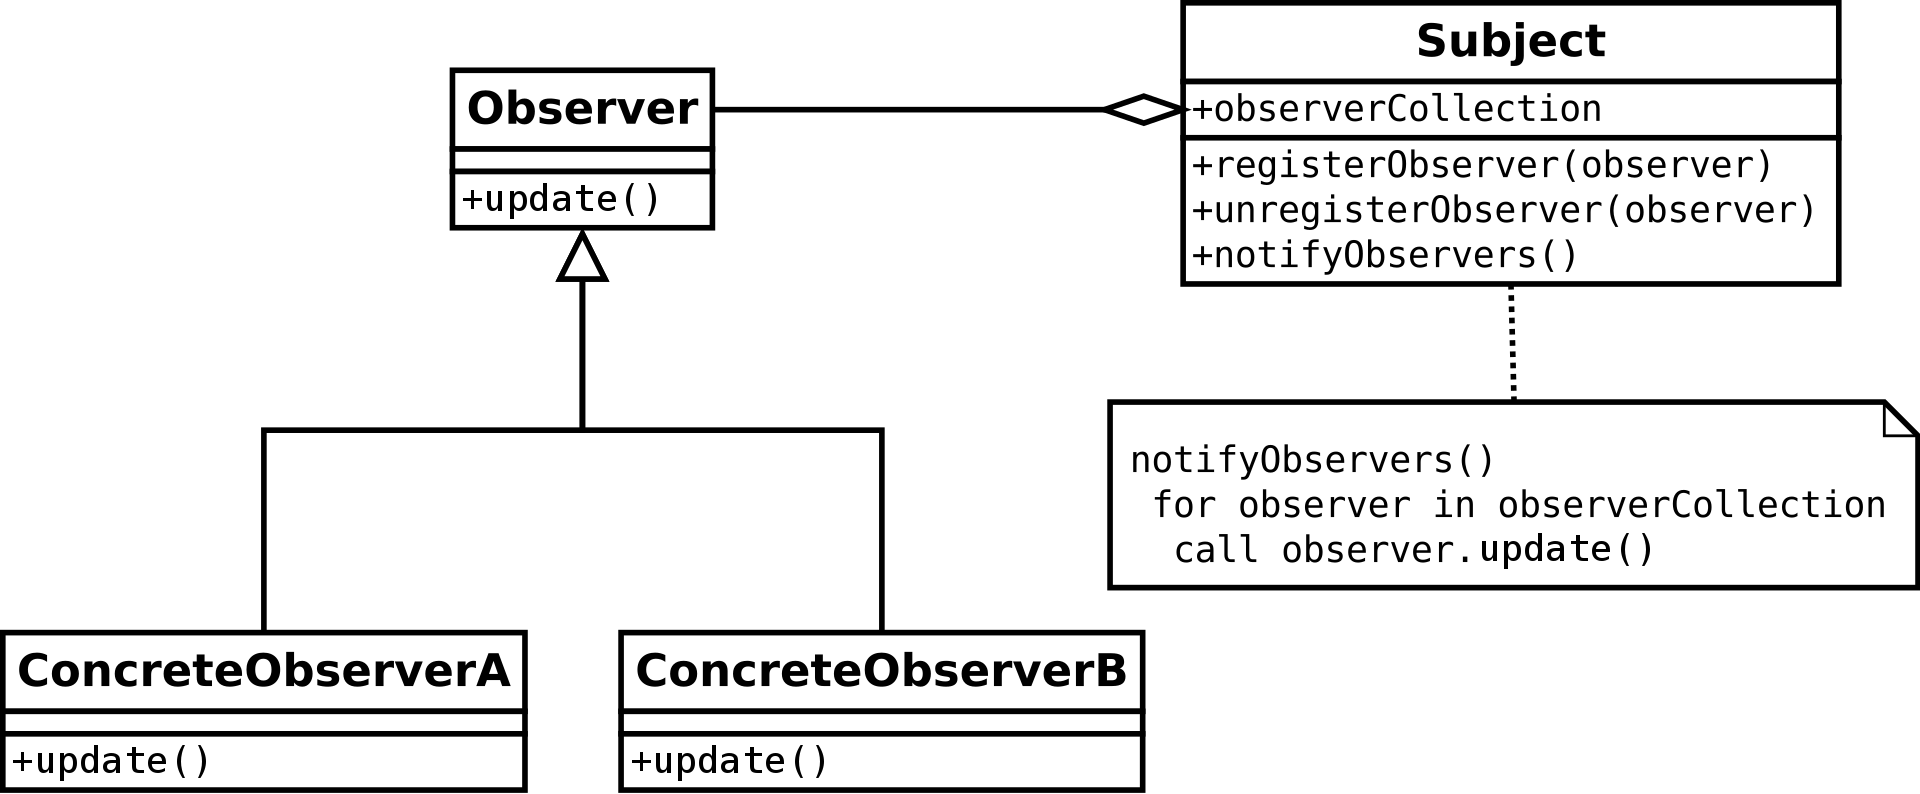
\includegraphics[width=0.8\textwidth]{Observer}

}

Un'alternativa al pattern observer, che però presenta alcune problematiche, è la \textit{callback relationship}.
La \textit{class-based callback relationship} inserisce un riferimento al \texttt{Subject} in ogni \texttt{Observer} e viceversa. 
Questo, però, porta a una dipendenza reciproca tra i \texttt{Subject} e tutti gli \texttt{Observer}.
La \textit{interface-based callback relationship} inserisce in ogni \texttt{Observer} un riferimento a una interfaccia \texttt{IObserverEvents}, che viene implementata dal \texttt{Subject}.
In questo modo \texttt{Subject} dipende da \texttt{Observer} ma non viceversa, perché \texttt{IObserverEvents} sta all'interno di \texttt{Observer}.
Tuttavia, questa relazione non permette a più \texttt{Observer} di osservare uno stesso \texttt{Subject}.

\end{solution}
\part Pattern MVC
\begin{solution}
Il pattern MVC divide un'applicazione in tre componenti: modello, view e controller.

Modello: gestisce un insieme di dati logicamente correlati; risponde alle interrogazioni sui dati; risponde alle istruzioni di modifica dello stato; genera un evento quando lo stato cambia; registra, in forma anonima, gli oggetti interessati alla notifica dell’evento.

View: gestisce un’area di visualizzazione, nella quale presenta all’utente una vista dei dati gestiti dal model; mappa i dati del model, o una parte, in oggetti visuali e visualizza tali oggetti su un particolare dispositivo di output; si registra presso il model per ricevere l’evento di cambiamento di stato.

Controller: gestisce gli input dell’utente (mouse, tastiera, etc.); mappa le azioni dell’utente nei comandi; invia tali comandi al model e/o alla view, che effettuano le operazioni appropriate.
\end{solution}
\part Pattern MVP
\begin{solution}
Il pattern MVP è una versione più "incapsulata" del pattern MVC, che favorisce il riuso delle view al costo di maggiore complessità.

Modello: gestisce un insieme di dati logicamente correlati; risponde alle interrogazioni sui dati; risponde alle istruzioni di modifica dello stato; genera un evento quando lo stato cambia; registra, in forma anonima, gli oggetti interessati alla notifica dell’evento.

View: gestisce un’area di visualizzazione, nella quale presenta all’utente una vista dei dati fornitele dal presenter; mappa i dati forniti dal presenter, o una parte, in oggetti visuali e visualizza tali oggetti su un particolare dispositivo di output; si registra presso il presenter per ricevere l’evento di cambiamento di stato.

Controller: gestisce gli input dell’utente (mouse, tastiera, etc.); mappa le azioni dell’utente nei comandi; invia tali comandi al model, che effettua le operazioni appropriate; aggiorna la view;
\end{solution}

\part Pattern flyweight
\begin{solution}

\textbf{Problema:} Si ha una serie di oggetti molto leggeri, ma nonostante la loro leggerezza non se ne vogliono istanziare tanti.

\textbf{Soluzione:} Si condividono gli oggetti, nascondendo la condivisione a tutti gli utilizzatori. 
Si usa un metodo factory che conserva un dizionario di Flyweight e invece di usare \texttt{new()} si chiama la factory, che cerca nel dizionario il flyweight corrispondente alla chiave e lo crea se e solo se non esiste.

\textbf{Conseguenze:} \begin{itemize}
\item l'oggetto flyweight non deve essere distinguibile da un oggetto non condiviso (quindi non può fare ipotesi sul contesto di utilizzazione).
\item i clienti non devono istanziare i propri flyweight, ma essi vanno creati tramite una factory
\item va esplicitata la distinzione tra stato intrinseco (che non dipende dal contesto e può essere condiviso) ed estrinseco (deve essere memorizzato dai clienti, che lo passano al flyweight)
\end{itemize}

\textbf{Diagramma UML}:

{\centering

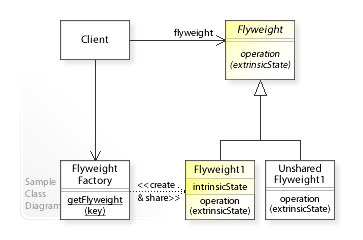
\includegraphics[width=0.8\textwidth]{Flyweight}

}


\end{solution}

\part Pattern strategy
\begin{solution}

\textbf{Problema:} Si hanno diverse possibilità per implementare un certo comportamento, e l'utilizzo di una di queste è indifferente.

\textbf{Soluzione:} Si dichiara una interfaccia che dichiara i metodi che svolgono la funzionalità richiesta, e si fa dipendere il client dall'interfaccia.

\textbf{Diagramma UML}:

{\centering

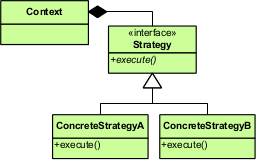
\includegraphics[width=0.8\textwidth]{Strategy}

}


\end{solution}

\part Pattern adapter/wrapper
\begin{solution}

\textbf{Problema:} Si vuole convertire l'interfaccia di una classe (\textit{adaptee}) in un'altra interfaccia che il cliente si aspetta.

\textbf{Soluzione:} Si scrive una classe che implementa l'interfaccia richiesta dal client e realizza le operazioni delegandone l'effettiva esecuzione a una istanza dell'\textit{adaptee}.

\textbf{Diagramma UML}:

{\centering

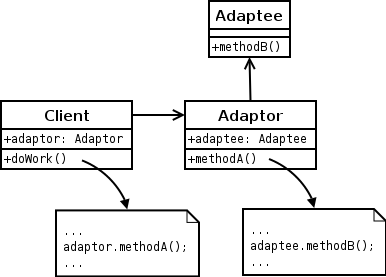
\includegraphics[width=0.8\textwidth]{Adapter}

}


\end{solution}

\part Pattern decorator
\begin{solution}

\textbf{Problema:} Si hanno molti comportamenti possibili e non si vuole creare un numero di sottoclassi che cresce esponenzialmente. 

\textbf{Soluzione:} Si scrive una interfaccia\texttt{IComponent}, implementata da\texttt{ConcreteComponent} e \texttt{Decorator}. 

\texttt{Decorator} è a sua volta astratta ed è specializzata dai vari \texttt{ConcreteDecorator} e ha un'associazione molti-a-uno con \texttt{IComponent} in modo da poter avere riferimenti innestati fino ad arrivare all'operazione base. 

\textbf{Diagramma UML}:

{\centering

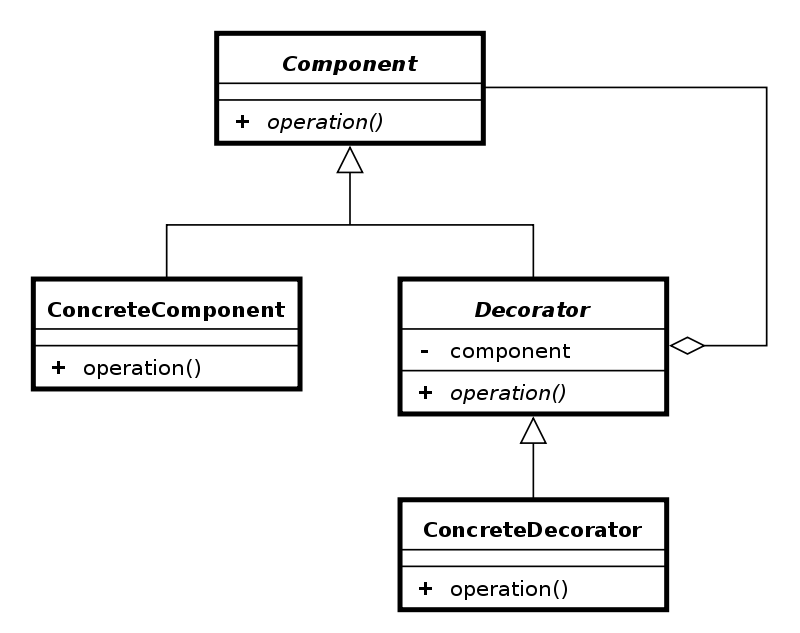
\includegraphics[width=0.8\textwidth]{Decorator}

}


\end{solution}

\part Pattern state
\begin{solution}

\textbf{Problema:} Si vuole che un oggetto cambi comportamento a seconda del suo stato, come se cambiasse classe durante l'esecuzione, cosa non possibile nella maggior parte dei linguaggi a oggetti.

\textbf{Soluzione:} Si associa il contesto a una classe astratta \texttt{AbstractState}, che rappresenta lo stato.
\texttt{AbstractState} è implementata dai vari \texttt{ConcreteState}, che hanno un metodo \texttt{HandleStateChange()}.
A ogni cambiamento di stato, il contesto chiama \texttt{Request()} che, per implementare il comportamento che dipende dallo stato, a sua volta chiama \texttt{HandleStateChange()} del proprio stato corrente, il quale può a sua volta richiamare un metodo \texttt{SetState()} del cliente per cambiarne lo stato.

\textbf{Diagramma UML}:

{\centering

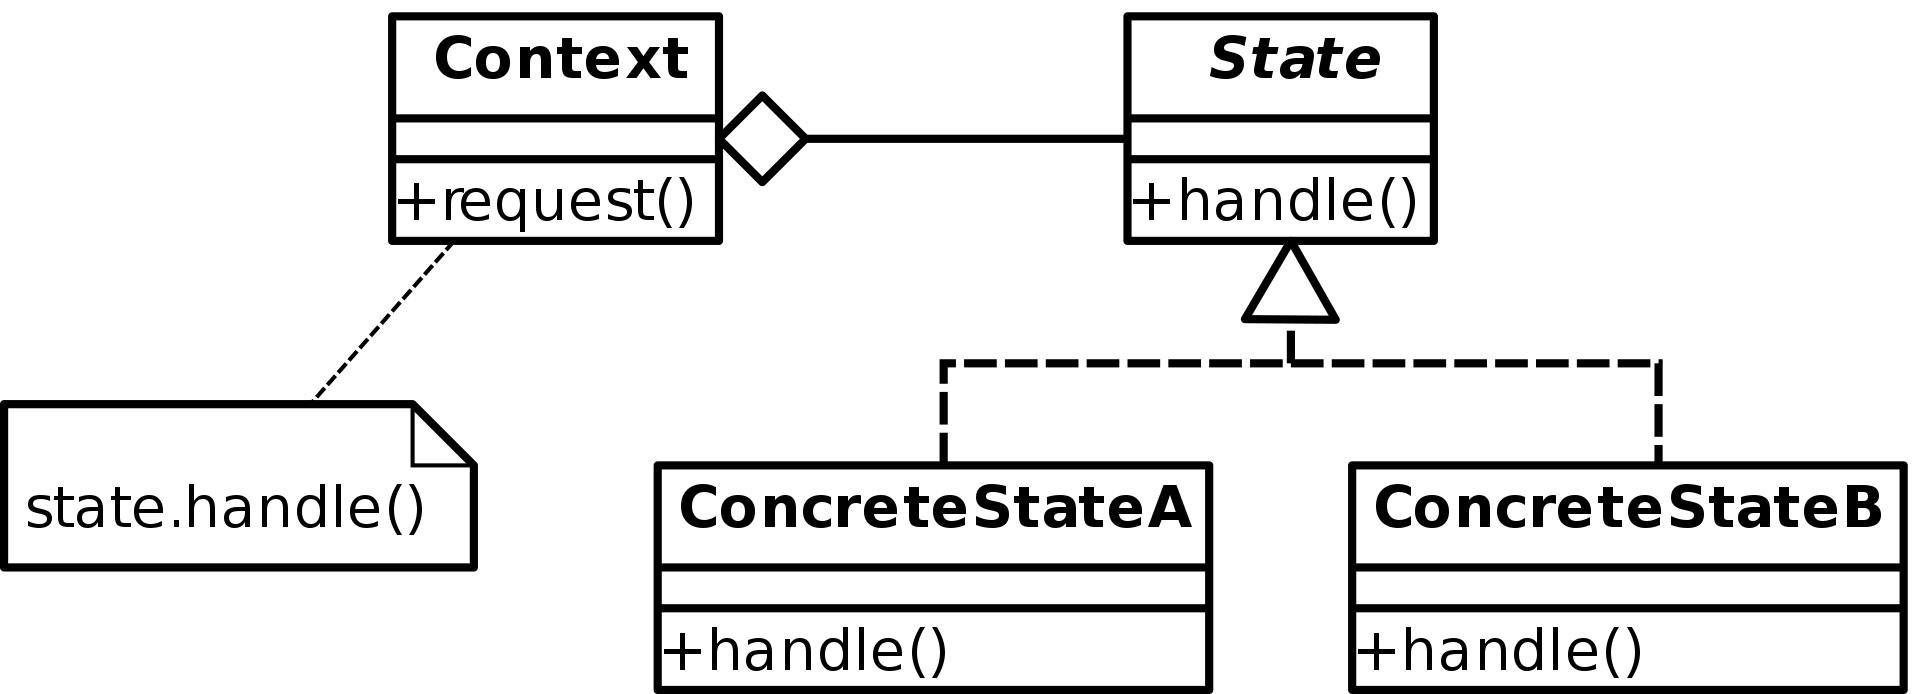
\includegraphics[width=0.8\textwidth]{State}

}


\end{solution}
\newpage
\part Pattern  composite
\begin{solution}

\textbf{Problema:} Si vuole rappresentare una gerarchia di contenitori e contenuti. È necessario poter navigare dal contenitore al contenuto e viceversa.

\textbf{Soluzione}: Si scrive una classe astratta \texttt{Component}, estesa da \texttt{Leaf}  (che non può avere figli) e \texttt{Composite}, che può avere figli.
Composite è quindi una composizione di \texttt{Component}. 
Ogni figlio ha un riferimento al genitore.

\textbf{Conseguenze:} Il contenitore dei figli deve essere un attributo di \texttt{Composite} (array, lista, hashtable ecc). 
Tutti gli elementi che hanno come genitore un componente devono essere figli, quindi diventa necessario aggiornare il padre quando si aggiornano i figli o viceversa (non entrambi per evitare un aggiornamento ciclico).

\textbf{Diagramma UML}:

{\centering

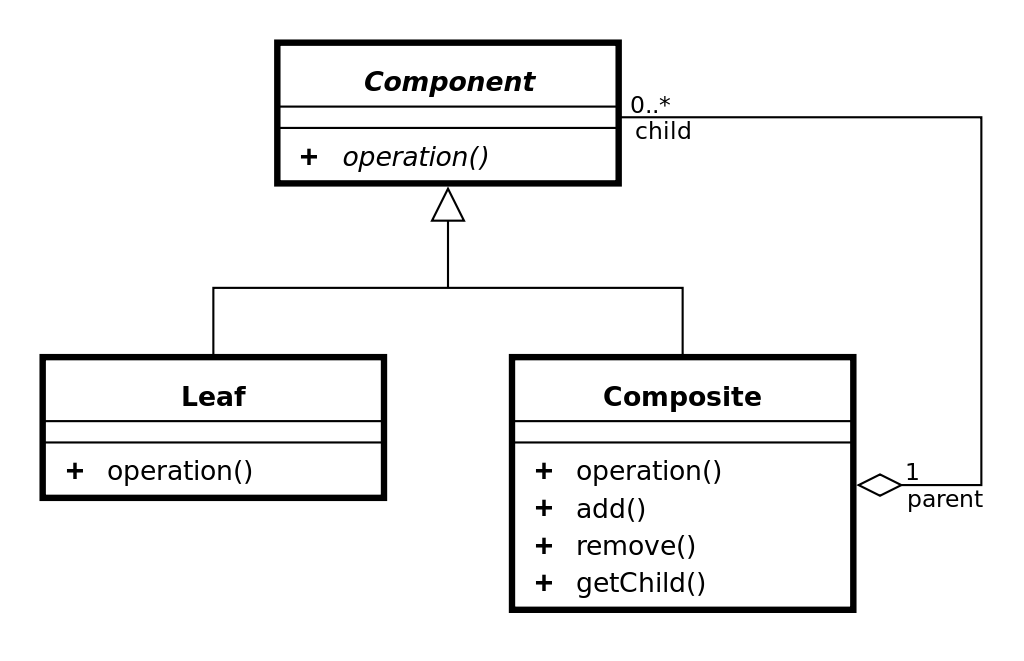
\includegraphics[width=0.8\textwidth]{Composite}

}


\end{solution}

\part Pattern visitor
\begin{solution}

\textbf{Problema:} Si vogliono effettuare varie operazioni sugli elementi di una struttura e queste operazioni non sono necessariamente note quando definisco la struttura stessa.

\textbf{Soluzione:} Si definisce una classe astratta \texttt{Visitor}.
Si creano nuove classi per ogni operazione, che estendono \texttt{Visitor}.
Si dichiara nella struttura un'operazione per accettare un generico \texttt{Visitor}. 

\textbf{Conseguenze:}
\begin{itemize}
    \item Si deve prestare attenzione all'incapsulamento, perché i \texttt{Visitor} devono poter accedere allo stato della struttura.
    \item Per ogni elemento concreto della struttura diventa necessario dichiarare un metodo \texttt{Visit()} in tutti i visitatori concreti, quindi la modifica della struttura ha un grosso impatto sui \texttt{Visitor}. La struttura deve quindi essere stabile.
    \item L'operazione effettuata è di tipo \textit{double dispatch}, perché dipende dal tipo di visitatore e visitato.
\end{itemize}

\textbf{Diagramma UML}:

{\centering

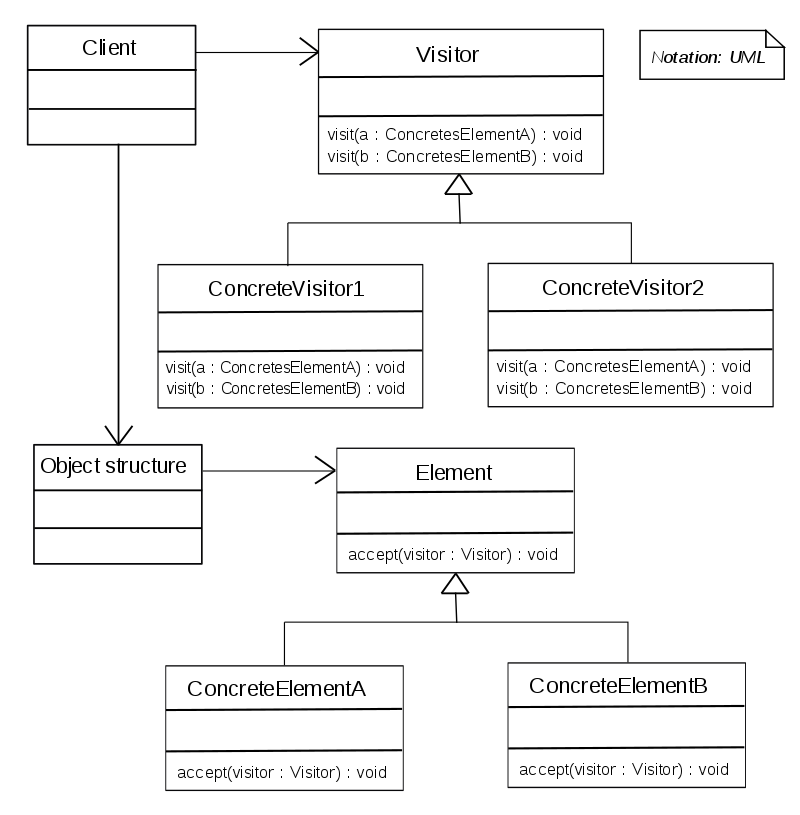
\includegraphics[width=0.8\textwidth]{Visitor}

}


\end{solution}


\end{parts}

\question \textbf{Sistemi di controllo delle versioni.}
\begin{parts}
\part Vantaggi e svantaggi del modello Lock-Modify-Unlock
\begin{solution}

Con l'uso di sistemi di controllo delle versioni, si può verificare la seguente situazione:
\begin{itemize}
    \item Utente A e B eseguono il check-out e lavorano sulle proprie working copy;
    \item Utente A esegue il check-in;
    \item Utente B esegue il check-in dopo di A, sovrascrivendo le modifiche di A.
\end{itemize}

Un modo per impedire il verificarsi di questa situazione, o almeno notificare quando avviene, è il modello Lock-Modify-Unlock (LMU), nel quale il sistema tiene traccia di chi stai modificando i vari file: ogni volta che qualcuno esegue il check-out e vuole modificare un file dichiara l'impostazione un lock su quel file, che non può essere modificato finché il lock non viene rilasciato.
Quando l'utente termina di modificare il file ed esegue il check-in, il lock viene rilasciato (unlock).
Questo presenta alcuni problemi:
\begin{itemize}
    \item Notevoli ritardi se ci si scorda di eseguire l'unlock di un file;
    \item Serializzazione superflua: se due utenti vogliono modificare parti diverse di un file, anche se le modifiche non si sovrappongono non è permesso lavorare su parti diverse di un file;
    \item Falso sentimento di sicurezza: il fatto che due utenti modifichino file diversi non vuol dire che le oro modifiche siano necessariamente indipendenti. 
    Se i due file che stanno venendo modificati dipendono l'uno dall'altro, potrebbero non funzionare come dovrebbero se le modifiche sono incompatibili;
    \item Richiede agli sviluppatori di essere costantemente online.
\end{itemize}

Questi problemi significano che l'unico caso in cui il modello LMU è preferibile al Copy-Modify-Merge è nel caso di file che non possono essere facilmente uniti, come ad esempio i file immagine.
\end{solution}
\part Vantaggi e svantaggi del modello Copy-Modify-Merge
\begin{solution}
Nel modello Copy-Modify-Merge (CMM) non ci sono lock, chiunque può modificare qualsiasi cosa, e al momento del check-in le modifiche effettuate dai vari utenti sono unite, non sovrascritte, tra di loro. 
Non è importante sapere quali sono gli altri utenti, ma solo quali modifiche hanno effettuato. 

Prima di poter eseguire il check-in, il sistema si accorge che le modifiche sono state effettuate partendo da una versione precedente del file e pretende che l'utente aggiorni il proprio file con tutte le modifiche effettuate dagli altri utenti nel frattempo. 
Questa operazione, chiamata \textit{merge}, può andare a buon fine o presentare conflitti: si hanno conflitti se l'applicazione delle modifiche non è simmetrica, cioè non è indifferente applicare prima o dopo le modifiche di uno qualunque degli utenti.
I conflitti vanno risolti a mano. 
Solitamente, in ogni caso, il tempo necessario per risolvere i conflitti è sensibilmente minore del tempo che si sarebbe perso adottando un modello a lock.

Nel caso in cui due utenti effettuino modifiche che sono sintatticamente compatibili ma rompono l'interazione semantica tra più moduli, il VCS non rileva alcun conflitto.
Il modello CMM non è quindi in grado di individuare i conflitti logici/concettuali/semantici. 


\end{solution}
\end{parts}

\end{questions}

Questo documento è rilasciato sotto licenza CC-BY-SA 4.0. \ccbysa

\end{document}
